% Options for packages loaded elsewhere
\PassOptionsToPackage{unicode}{hyperref}
\PassOptionsToPackage{hyphens}{url}
\PassOptionsToPackage{dvipsnames,svgnames,x11names}{xcolor}
\documentclass[
  10pt]{article}
\usepackage{xcolor}
\usepackage[margin=19mm]{geometry}
\usepackage{amsmath,amssymb}
\setcounter{secnumdepth}{-\maxdimen} % remove section numbering
\usepackage{iftex}
\ifPDFTeX
  \usepackage[T1]{fontenc}
  \usepackage[utf8]{inputenc}
  \usepackage{textcomp} % provide euro and other symbols
\else % if luatex or xetex
  \usepackage{unicode-math} % this also loads fontspec
  \defaultfontfeatures{Scale=MatchLowercase}
  \defaultfontfeatures[\rmfamily]{Ligatures=TeX,Scale=1}
\fi
\usepackage{lmodern}
\ifPDFTeX\else
  % xetex/luatex font selection
    \setmainfont[]{TeX Gyre Termes}
\fi
% Use upquote if available, for straight quotes in verbatim environments
\IfFileExists{upquote.sty}{\usepackage{upquote}}{}
\IfFileExists{microtype.sty}{% use microtype if available
  \usepackage[]{microtype}
  \UseMicrotypeSet[protrusion]{basicmath} % disable protrusion for tt fonts
}{}
\makeatletter
\@ifundefined{KOMAClassName}{% if non-KOMA class
  \IfFileExists{parskip.sty}{%
    \usepackage{parskip}
  }{% else
    \setlength{\parindent}{0pt}
    \setlength{\parskip}{6pt plus 2pt minus 1pt}}
}{% if KOMA class
  \KOMAoptions{parskip=half}}
\makeatother
\usepackage{longtable,booktabs,array}
\usepackage{calc} % for calculating minipage widths
% Correct order of tables after \paragraph or \subparagraph
\usepackage{etoolbox}
\makeatletter
\patchcmd\longtable{\par}{\if@noskipsec\mbox{}\fi\par}{}{}
\makeatother
% Allow footnotes in longtable head/foot
\IfFileExists{footnotehyper.sty}{\usepackage{footnotehyper}}{\usepackage{footnote}}
\makesavenoteenv{longtable}
\usepackage{graphicx}
\makeatletter
\newsavebox\pandoc@box
\newcommand*\pandocbounded[1]{% scales image to fit in text height/width
  \sbox\pandoc@box{#1}%
  \Gscale@div\@tempa{\textheight}{\dimexpr\ht\pandoc@box+\dp\pandoc@box\relax}%
  \Gscale@div\@tempb{\linewidth}{\wd\pandoc@box}%
  \ifdim\@tempb\p@<\@tempa\p@\let\@tempa\@tempb\fi% select the smaller of both
  \ifdim\@tempa\p@<\p@\scalebox{\@tempa}{\usebox\pandoc@box}%
  \else\usebox{\pandoc@box}%
  \fi%
}
% Set default figure placement to htbp
\def\fps@figure{htbp}
\makeatother
\setlength{\emergencystretch}{3em} % prevent overfull lines
\providecommand{\tightlist}{%
  \setlength{\itemsep}{0pt}\setlength{\parskip}{0pt}}
\usepackage{booktabs}
\usepackage{longtable}
\usepackage{array}
\usepackage{microtype}
\usepackage{setspace}
\setstretch{1.12}
\setlength{\emergencystretch}{3em}
\setlength{\parindent}{0pt}
\setlength{\parskip}{0.45em}
\usepackage{caption}
\captionsetup{font=small,labelfont=bf}
\usepackage{needspace}
\usepackage{etoolbox}
\AtBeginEnvironment{longtable}{\small}
\usepackage{bookmark}
\IfFileExists{xurl.sty}{\usepackage{xurl}}{} % add URL line breaks if available
\urlstyle{same}
\hypersetup{
  pdftitle={Supplementary information for A traceable time-series power-flow dataset for Portugal's high-voltage grid},
  colorlinks=true,
  linkcolor={Maroon},
  filecolor={Maroon},
  citecolor={Blue},
  urlcolor={Blue},
  pdfcreator={LaTeX via pandoc}}

\title{Supplementary information for A traceable time-series power-flow
dataset for Portugal's high-voltage grid}
\author{}
\date{}

\begin{document}
\maketitle

This document supplements the Data Descriptor. Machine-readable field
definitions, device-level audits, complete contingency membership, file
hashes, and replay commands are provided in the versioned release data
dictionary, CSV/JSON audit products, and release manifest.

\textbf{Table S1 \textbar{} Mapping from source fields to standardized
semantics.}

\begin{longtable}[]{@{}
  >{\raggedright\arraybackslash}p{(\linewidth - 6\tabcolsep) * \real{0.2500}}
  >{\raggedright\arraybackslash}p{(\linewidth - 6\tabcolsep) * \real{0.2500}}
  >{\raggedright\arraybackslash}p{(\linewidth - 6\tabcolsep) * \real{0.2500}}
  >{\raggedright\arraybackslash}p{(\linewidth - 6\tabcolsep) * \real{0.2500}}@{}}
\toprule\noalign{}
\begin{minipage}[b]{\linewidth}\raggedright
Source / source field
\end{minipage} & \begin{minipage}[b]{\linewidth}\raggedright
Standard meaning or target field
\end{minipage} & \begin{minipage}[b]{\linewidth}\raggedright
Transformation
\end{minipage} & \begin{minipage}[b]{\linewidth}\raggedright
Join and missing-data rule
\end{minipage} \\
\midrule\noalign{}
\endhead
\bottomrule\noalign{}
\endlastfoot
E-REDES \texttt{energia} & Nodal \texttt{p\_mw} & 15-min kWh / 250 to MW
& Match \texttt{codigo\_subestacao} to facility; no interpolation \\
E-REDES \texttt{datahora}; \texttt{data} / \texttt{hora} & UTC interval
start & Subtract 15 min from end label; Europe/Lisbon to UTC & Average
duplicate labels by station and flag ambiguity \\
REN \texttt{source\_date} + \texttt{source\_index} &
\texttt{calendar.timestamp\_utc} & Construct from Lisbon civil date and
within-day index & Index distinguishes repeated daylight-saving hour \\
REN \texttt{series\_name} + \texttt{value\_mw} & National total by
energy, load, or storage type & Preserve MW; allocate within type &
Missing required series fails the case \\
RND line ID / \texttt{tensao\_de} & \texttt{source\_line\_id} /
\texttt{voltage\_kv} & Preserve source key; standardize voltage to kV &
Restrict to voltage levels in this release \\
Source geometry / coordinates & Geospatial geometry; longitude /
latitude & Store in WGS 84; compute distances in EPSG:3763 & Invalid
geometry is recorded \\
OSM way / relation / power tags & Source ID, circuit identity, asset
type & Split only at explicit nodes; retain relation keys & Geometric
crossing does not imply connection \\
Public nameplate capacity and rating & \texttt{nameplate\_mw} /
\texttt{sn\_mva} & Standardize power and capacity units & Missing public
value uses a flagged proxy \\
Archived URL / bytes / hash & \texttt{provenance.raw\_files} & SHA-256
and relative archive path & Retain source-file locator \\
\end{longtable}

The table describes semantic mappings and does not imply identical raw
field names in every source file. The archived source files remain
authoritative for exact raw fields.

\textbf{Table S2 \textbar{} Default electrical-parameter library.}

\begin{longtable}[]{@{}
  >{\raggedleft\arraybackslash}p{(\linewidth - 10\tabcolsep) * \real{0.1739}}
  >{\raggedleft\arraybackslash}p{(\linewidth - 10\tabcolsep) * \real{0.1739}}
  >{\raggedleft\arraybackslash}p{(\linewidth - 10\tabcolsep) * \real{0.1739}}
  >{\raggedleft\arraybackslash}p{(\linewidth - 10\tabcolsep) * \real{0.1739}}
  >{\raggedleft\arraybackslash}p{(\linewidth - 10\tabcolsep) * \real{0.1739}}
  >{\raggedright\arraybackslash}p{(\linewidth - 10\tabcolsep) * \real{0.1304}}@{}}
\toprule\noalign{}
\begin{minipage}[b]{\linewidth}\raggedleft
Voltage (kV)
\end{minipage} & \begin{minipage}[b]{\linewidth}\raggedleft
r (Ω/km)
\end{minipage} & \begin{minipage}[b]{\linewidth}\raggedleft
x (Ω/km)
\end{minipage} & \begin{minipage}[b]{\linewidth}\raggedleft
c (nF/km)
\end{minipage} & \begin{minipage}[b]{\linewidth}\raggedleft
Imax (kA)
\end{minipage} & \begin{minipage}[b]{\linewidth}\raggedright
Status
\end{minipage} \\
\midrule\noalign{}
\endhead
\bottomrule\noalign{}
\endlastfoot
60 & 0.1093 & 0.368854 & 9.2 & 0.606 & Voltage-class engineering
proxy \\
130 & 0.07 & 0.33 & 9.8 & 0.8 & Voltage-class engineering proxy \\
150 & 0.06 & 0.32 & 10.0 & 0.85 & Voltage-class engineering proxy \\
220 & 0.04 & 0.285 & 11.0 & 1.2 & Voltage-class engineering proxy \\
400 & 0.025 & 0.25 & 12.0 & 2.0 & Voltage-class engineering proxy \\
\end{longtable}

These are summer baseline defaults rather than final values for every
line. Source-backed values override individual fields. Cable factors are
r ×0.65, x ×0.35, c ×20, and Imax ×0.90; seasonal rating factors are
given in Table 6 of the main manuscript. Values are frozen in
\texttt{model\_config.json}.

\begin{longtable}[]{@{}lrrr@{}}
\toprule\noalign{}
Transformer voltage pair (kV) & Default S (MVA) & vk (\%) & vkr (\%) \\
\midrule\noalign{}
\endhead
\bottomrule\noalign{}
\endlastfoot
400/220 & 450.0 & 12.0 & 0.3 \\
400/150 & 450.0 & 12.0 & 0.3 \\
400/60 & 170.0 & 12.0 & 0.35 \\
220/150 & 250.0 & 12.0 & 0.35 \\
150/130 & 140.0 & 12.0 & 0.45 \\
220/60 & 170.0 & 12.0 & 0.4 \\
150/60 & 170.0 & 12.0 & 0.45 \\
130/60 & 126.0 & 12.0 & 0.45 \\
\end{longtable}

Default transformer capacities and impedances are engineering proxies.
Published capacities take precedence. When aggregate capacity for a
voltage pair is lower than the REN inventory, capacities are scaled
upward and the factor is retained. Device-specific overrides, including
Estoi, take precedence over these defaults.

\textbf{Table S3 \textbar{} Principal mapping and evidence fields.}

\begin{longtable}[]{@{}
  >{\raggedright\arraybackslash}p{(\linewidth - 4\tabcolsep) * \real{0.3333}}
  >{\raggedright\arraybackslash}p{(\linewidth - 4\tabcolsep) * \real{0.3333}}
  >{\raggedright\arraybackslash}p{(\linewidth - 4\tabcolsep) * \real{0.3333}}@{}}
\toprule\noalign{}
\begin{minipage}[b]{\linewidth}\raggedright
Storage location
\end{minipage} & \begin{minipage}[b]{\linewidth}\raggedright
Principal fields
\end{minipage} & \begin{minipage}[b]{\linewidth}\raggedright
Interpretation
\end{minipage} \\
\midrule\noalign{}
\endhead
\bottomrule\noalign{}
\endlastfoot
\texttt{grid.generators} & \texttt{source\_id}; \texttt{bus\_id};
\texttt{bus\_assignment\_rule}; \texttt{available\_from\_utc} & Asset
source, bus mapping, and commissioning treatment \\
\texttt{grid.buses} & \texttt{endpoint\_match\_distance\_m};
\texttt{source\_status} & Source-backed versus derived buses \\
\texttt{grid.lines} & \texttt{parameter\_status};
\texttt{r/x/c/max\_i\_status} & Field-level parameter evidence \\
\texttt{scenario.load\_operating\_points} & \texttt{observed\_p\_mw};
\texttt{ren\_residual\_p\_mw}; \texttt{q\_mvar} & Observed load and
spatially allocated residual \\
\texttt{monthly\_model.audit\_bundles} & Allocation, boundary, and loss
records & Case-level conservation audit \\
\texttt{provenance.raw\_record\_locator} & \texttt{entity\_id};
\texttt{raw\_table}; \texttt{raw\_record\_id} & Link from derived entity
to source record \\
\end{longtable}

\textbf{Table S4 \textbar{} Quality controls and failure handling.}

\begin{longtable}[]{@{}
  >{\raggedright\arraybackslash}p{(\linewidth - 6\tabcolsep) * \real{0.2500}}
  >{\raggedright\arraybackslash}p{(\linewidth - 6\tabcolsep) * \real{0.2500}}
  >{\raggedright\arraybackslash}p{(\linewidth - 6\tabcolsep) * \real{0.2500}}
  >{\raggedright\arraybackslash}p{(\linewidth - 6\tabcolsep) * \real{0.2500}}@{}}
\toprule\noalign{}
\begin{minipage}[b]{\linewidth}\raggedright
Layer / check
\end{minipage} & \begin{minipage}[b]{\linewidth}\raggedright
Threshold or condition
\end{minipage} & \begin{minipage}[b]{\linewidth}\raggedright
Action
\end{minipage} & \begin{minipage}[b]{\linewidth}\raggedright
Record location
\end{minipage} \\
\midrule\noalign{}
\endhead
\bottomrule\noalign{}
\endlastfoot
Static / identifiers and endpoints & Valid equipment key and existing
endpoints & Block invalid connection & Static audit and provenance \\
Static / voltage and length & Same-voltage connection, length
\textgreater0, no self-loop & Block invalid branch & Topology audit \\
Static / connectivity & Components, isolated nodes, boundary inventory &
Record and interpret within scope & \texttt{topology\_summary.json} \\
Time series / required inputs & Consistent UTC keys and required series
present & Retain error; do not interpolate &
\texttt{monthly\_model.cases.error} \\
Time series / load conservation & Nodal sum differs from Consumption +
Storage by ≤0.11 MW & Block case if failed & Allocation audit \\
Time series / generation capacity & Commissioned mapped assets satisfy
0≤P≤nameplate & Excess becomes an explicit national proxy &
Generation-allocation audit \\
Solution / AC convergence & Newton--Raphson tolerance \(10^{-6}\) MVA;
≤50 iterations & Retain failed status & \texttt{monthly\_model.cases} \\
Solution / active-power closure & Record Pgen + Pnet − Pload − Ploss &
Report numerical residual & Audit bundle and validation summary \\
Screening / voltage and thermal & 0.90--1.10 p.u.; normally 100\% rating
& Flag; retain completed case & Cases and state arrays \\
External comparison & Common time or region; pairwise missing exclusion
& Retain anomalous months and report n & Comparison output and
confidence intervals \\
Database write & Summary, arrays, and audit bundle in one transaction &
Roll back full case and retain error & Monthly transaction log \\
Release integrity & Expected, complete, array, and audit counts agree &
Do not mark month complete if failed & Run manifest and hashes \\
\end{longtable}

Contingency thresholds and exclusions are defined in Table S8; routine
case-quality checks and contingency screening are distinct.

\section{Supplementary Notes}\label{supplementary-notes}

\subsection{Supplementary Note S1 \textbar{} Data layers and
joins}\label{supplementary-note-s1-data-layers-and-joins}

\textbf{Table S5 \textbar{} Data layers, grain, and principal join
keys.}

\begin{longtable}[]{@{}
  >{\raggedright\arraybackslash}p{(\linewidth - 6\tabcolsep) * \real{0.2500}}
  >{\raggedright\arraybackslash}p{(\linewidth - 6\tabcolsep) * \real{0.2500}}
  >{\raggedright\arraybackslash}p{(\linewidth - 6\tabcolsep) * \real{0.2500}}
  >{\raggedright\arraybackslash}p{(\linewidth - 6\tabcolsep) * \real{0.2500}}@{}}
\toprule\noalign{}
\begin{minipage}[b]{\linewidth}\raggedright
Data layer
\end{minipage} & \begin{minipage}[b]{\linewidth}\raggedright
Grain
\end{minipage} & \begin{minipage}[b]{\linewidth}\raggedright
Principal join keys
\end{minipage} & \begin{minipage}[b]{\linewidth}\raggedright
Purpose
\end{minipage} \\
\midrule\noalign{}
\endhead
\bottomrule\noalign{}
\endlastfoot
\texttt{provenance.raw\_files} / \texttt{raw\_*} & File / source record
& \texttt{artifact\_id}; \texttt{raw\_record\_id} & Source evidence and
fingerprints \\
\texttt{grid.*} & Equipment & \texttt{model\_id}; equipment ID;
\texttt{bus\_id} & Static network and asset mapping \\
\texttt{geo.*} & Geometry & Equipment or facility ID & Spatial
representation \\
\texttt{main.interval\_calendar} / \texttt{ren\_dispatch} /
\texttt{eredes\_load} & 15-min interval or raw record &
\texttt{timestamp\_utc}; source time key & Common time-series inputs \\
Scenario operating-point tables & Time × equipment & \texttt{model\_id};
equipment ID; time key & Nodal inputs and boundary \\
\texttt{monthly\_model.cases} / \texttt{state\_arrays} & Case / case
array & \texttt{case\_id}; \texttt{timestamp\_utc} & State summary and
equipment results \\
Monthly audit bundles / \texttt{run\_manifest} & Case / monthly run &
\texttt{case\_id}; \texttt{run\_id} & Allocation audit and integrity \\
\texttt{raw\_eredes\_aux} / \texttt{scenario.annual\_nminus1\_*} &
Validation or contingency case & Region, facility, or time × element key
& External validation and examples \\
\end{longtable}

\subsection{Supplementary Note S2 \textbar{} Release and model-version
reconciliation}\label{supplementary-note-s2-release-and-model-version-reconciliation}

The unique frozen snapshot is \textbf{SimPT60-2026.09.21-r1}. CORE-3783
fixes the static network used for the 31,492 historical cases and the
main Technical Validation: 3,783 buses, 4,943 line rows, and 228
transformer rows. N1-3787 is restricted to the contingency examples in
Supplementary Notes S4--S5.

N1-3787 adds four colocated connection nodes to split the
Lanheses--Feitosa topology representation and reconnects the endpoints
of five lines without changing the line-row count. It retains 228
transformer rows. In the Estoi row, the \texttt{parallel} field changes
from one to three and per-unit \texttt{sn\_mva} from 170 to 126 MVA, so
the model represents 230 equivalent transformer units while preserving
228 transformer rows and 228 transformer outage groups. An Estoi unit
outage decrements \texttt{parallel} from three to two. The
representation does not establish that all three physical units were
simultaneously in service at every study time.

The differences were not written back to the historical monthly
databases. Users must select a named model variant for each analysis.
Field-level differences, static and asset SHA-256 hashes, the locked
environment, minimal replay command, and 22 regression snapshots are
stored in \texttt{release.json}, \texttt{SHA256SUMS}, the release
README, and \texttt{model\_field\_diff.csv}.

\subsection{Supplementary Note S3 \textbar{} Additional validation and
sensitivity}\label{supplementary-note-s3-additional-validation-and-sensitivity}

Parameter and spatial-allocation experiments use 22 representative
times. Table S6 gives paired statistics; Figure 5 in the main manuscript
shows the rank, Top-20 set, and maximum-loading responses.

\textbf{Table S6 \textbar{} Parameter and spatial-allocation
sensitivity.}

\begin{longtable}[]{@{}
  >{\raggedright\arraybackslash}p{(\linewidth - 10\tabcolsep) * \real{0.1304}}
  >{\raggedleft\arraybackslash}p{(\linewidth - 10\tabcolsep) * \real{0.1739}}
  >{\raggedleft\arraybackslash}p{(\linewidth - 10\tabcolsep) * \real{0.1739}}
  >{\raggedleft\arraybackslash}p{(\linewidth - 10\tabcolsep) * \real{0.1739}}
  >{\raggedleft\arraybackslash}p{(\linewidth - 10\tabcolsep) * \real{0.1739}}
  >{\raggedleft\arraybackslash}p{(\linewidth - 10\tabcolsep) * \real{0.1739}}@{}}
\toprule\noalign{}
\begin{minipage}[b]{\linewidth}\raggedright
Configuration
\end{minipage} & \begin{minipage}[b]{\linewidth}\raggedleft
Converged / cases
\end{minipage} & \begin{minipage}[b]{\linewidth}\raggedleft
Median / minimum ρ
\end{minipage} & \begin{minipage}[b]{\linewidth}\raggedleft
Median / minimum Jaccard
\end{minipage} & \begin{minipage}[b]{\linewidth}\raggedleft
Maximum absolute Δ loading (pp)
\end{minipage} & \begin{minipage}[b]{\linewidth}\raggedleft
Median absolute Δ loss rate (pp)
\end{minipage} \\
\midrule\noalign{}
\endhead
\bottomrule\noalign{}
\endlastfoot
Shared baseline & 22 / 22 & 1.000 / 1.000 & 1.000 / 1.000 & 0.00 &
0.000 \\
R/X +20\%; C −20\% & 22 / 22 & 0.9988 / 0.9985 & 0.905 / 0.739 & 6.08 &
0.284 \\
R/X −20\%; C +20\% & 22 / 22 & 0.9981 / 0.9977 & 0.905 / 0.739 & 6.56 &
0.278 \\
Current rating +20\% & 22 / 22 & 1.0000 / 1.0000 & 1.000 / 1.000 & 22.98
& 0.000 \\
Current rating −20\% & 22 / 22 & 1.0000 / 1.0000 & 1.000 / 1.000 & 34.48
& 0.000 \\
Transformer S −20\%, Z +20\% & 22 / 22 & 0.9948 / 0.9931 & 0.779 / 0.600
& 17.10 & 0.087 \\
Transformer S +20\%, Z −20\% & 22 / 22 & 0.9954 / 0.9950 & 0.818 / 0.538
& 13.78 & 0.058 \\
Uniform boundary weights & 22 / 22 & 0.9971 / 0.9939 & 0.905 / 0.667 &
17.37 & 0.183 \\
Voltage-weighted boundary & 22 / 22 & 0.9967 / 0.9936 & 1.000 / 0.739 &
7.81 & 0.089 \\
Same-technology capacity allocation & 22 / 22 & 0.9937 / 0.9642 & 1.000
/ 0.818 & 1.49 & 0.023 \\
Residual load by transformer capacity & 22 / 22 & 0.9962 / 0.9947 &
0.818 / 0.429 & 6.50 & 0.096 \\
Residual load uniform by delivery point & 22 / 22 & 0.9963 / 0.9952 &
0.905 / 0.538 & 9.91 & 0.086 \\
\end{longtable}

Each configuration uses 22 times. After removing the repeated baseline,
all 264 cases converged. Loss rate is network loss divided by model
load; changes are percentage points.

Hotspot persistence is computed within each time across 12
configurations. Seventy-four of 4,943 lines enter the Top 20 at least
once, and 56 reach a within-time frequency of at least 0.8. The highest
frequency across all experiments is 207/264=78.4\%; no line appears at
every time and configuration.

\pandocbounded{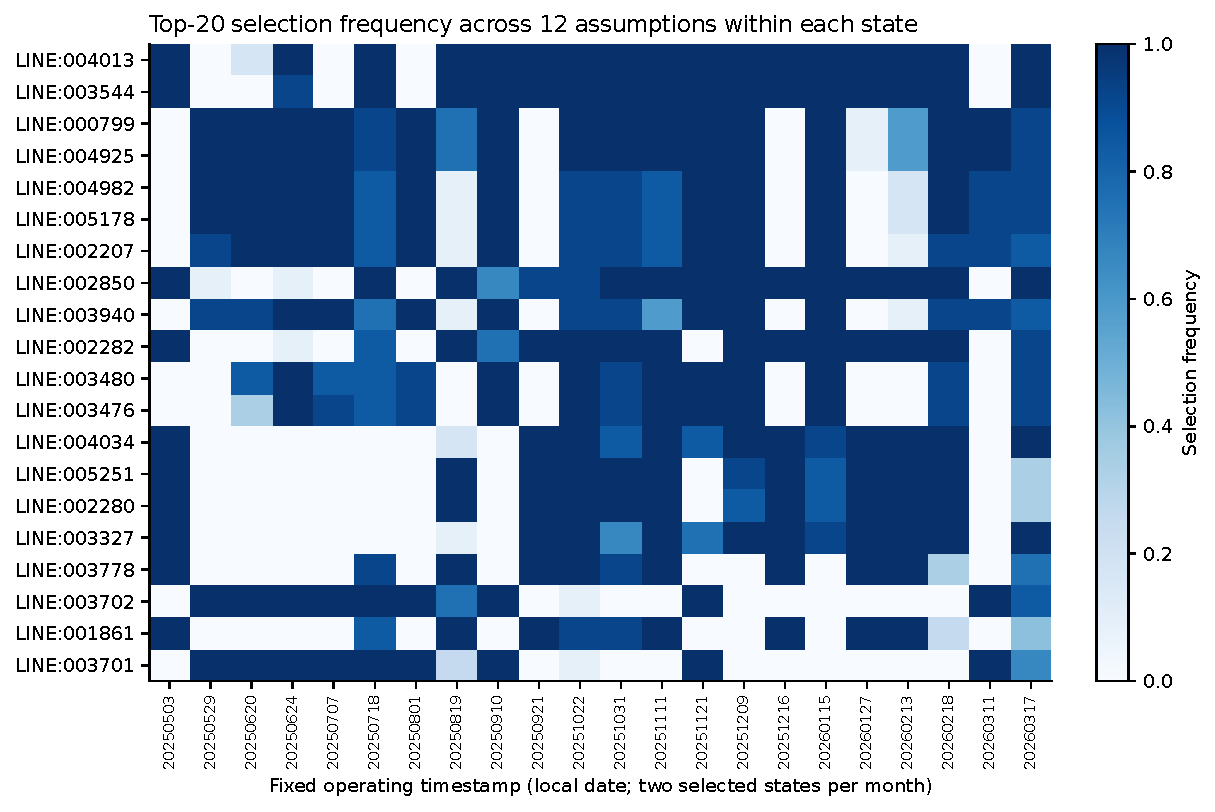
\includegraphics[keepaspectratio]{figures_final/fig06_hotspot_persistence.pdf}}

\textbf{Figure S1 \textbar{} Hotspot inclusion frequency under
alternative assumptions.} Each cell gives the proportion of the 12
configurations at one time in which a line enters the Top 20. Complete
membership and frequencies are released as CSV.

The station-held-out experiment uses substations as five deterministic
folds and compares global capacity share, five nearest geographic
stations, and five nearest stations on the reconstructed network.
Inverse distance weights are used; network distance uses in-service line
lengths and a small positive transformer-edge length. Confidence
intervals use a station-cluster bootstrap.

The operating-proxy ablation changes reactive-power limits, PV voltage
targets, load compensation, shunt reactors, and tap control at the same
22 times. Table S7 reports the largest paired changes relative to the
archived baseline.

\textbf{Table S7 \textbar{} Operating-proxy ablation; maximum absolute
change over 22 paired times.}

\begin{longtable}[]{@{}
  >{\raggedright\arraybackslash}p{(\linewidth - 8\tabcolsep) * \real{0.1579}}
  >{\raggedleft\arraybackslash}p{(\linewidth - 8\tabcolsep) * \real{0.2105}}
  >{\raggedleft\arraybackslash}p{(\linewidth - 8\tabcolsep) * \real{0.2105}}
  >{\raggedleft\arraybackslash}p{(\linewidth - 8\tabcolsep) * \real{0.2105}}
  >{\raggedleft\arraybackslash}p{(\linewidth - 8\tabcolsep) * \real{0.2105}}@{}}
\toprule\noalign{}
\begin{minipage}[b]{\linewidth}\raggedright
Configuration
\end{minipage} & \begin{minipage}[b]{\linewidth}\raggedleft
Converged / attempted
\end{minipage} & \begin{minipage}[b]{\linewidth}\raggedleft
Δ minimum voltage (p.u.)
\end{minipage} & \begin{minipage}[b]{\linewidth}\raggedleft
Δ maximum line loading (pp)
\end{minipage} & \begin{minipage}[b]{\linewidth}\raggedleft
Δ maximum transformer loading (pp)
\end{minipage} \\
\midrule\noalign{}
\endhead
\bottomrule\noalign{}
\endlastfoot
Baseline & 22 / 22 & 0.00000 & 0.000 & 0.000 \\
Legacy fixed neutral tap & 22 / 22 & 0.00000 & 0.000 & 0.000 \\
No compensation/reactors; fixed taps & 22 / 22 & 0.00917 & 0.248 &
0.892 \\
No load compensation & 22 / 22 & 0.00956 & 0.182 & 0.890 \\
Five reactors disabled & 22 / 22 & 0.00090 & 0.229 & 0.176 \\
PV target 0.99 & 22 / 22 & 0.01120 & 1.370 & 0.762 \\
PV target 1.01 & 22 / 22 & 0.01117 & 1.337 & 0.740 \\
Reactive-power limits ×1.5 & 22 / 22 & 0.00975 & 0.351 & 0.489 \\
Reactive-power limits ×0.5 & 22 / 22 & 0.02845 & 1.419 & 0.423 \\
Ratio taps active with voltage control & 22 / 22 & 0.00903 & 0.032 &
4.305 \\
Ratio taps active but fixed neutral & 22 / 22 & 0.00000 & 0.000 &
0.000 \\
\end{longtable}

\subsection{Supplementary Note S4 \textbar{} Detailed contingency
diagnostics}\label{supplementary-note-s4-detailed-contingency-diagnostics}

At one stressed snapshot, targeted diagnostics screen 50 highly loaded
physical line circuits and 20 in-service transformers. Sixty-seven of 70
cases converge under the specified reactive-power boundary and 66 pass
all screens. Three northern line cases yield diagnostic solutions only
after relaxing the reactive-power boundary and show thermal violations;
one radial circuit creates a material supply-loss island.

\pandocbounded{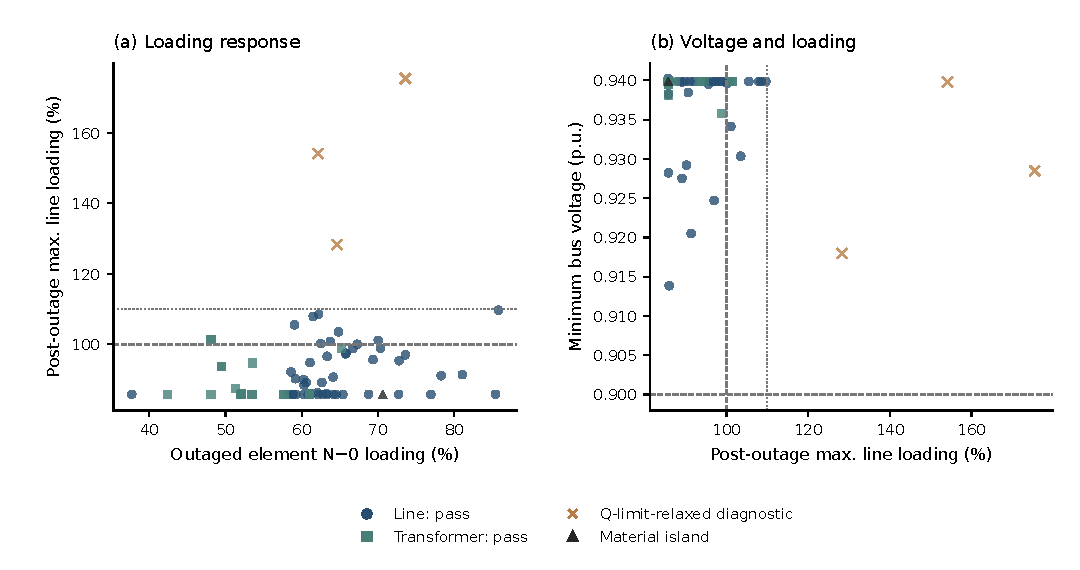
\includegraphics[keepaspectratio]{figures_final/fig10_targeted_nminus1.pdf}}

\textbf{Figure S2 \textbar{} Targeted AC N−1 response.} Circles and
squares denote line and transformer cases that pass screening; crosses
denote diagnostic-only solutions; triangles denote material islands.
Dashed lines show continuous-rating and voltage-screening limits.

The full-element panel uses the same 1,649 outage groups at all six
times. Table S8 defines selection and exclusion;
\texttt{nminus1\_exclusions.csv} and the result database contain
identifiers, membership hashes, endpoint state, and case-level output.

\textbf{Table S8 \textbar{} N−1 outage universe at the representative
times.}

\begin{longtable}[]{@{}
  >{\raggedright\arraybackslash}p{(\linewidth - 4\tabcolsep) * \real{0.3000}}
  >{\raggedleft\arraybackslash}p{(\linewidth - 4\tabcolsep) * \real{0.4000}}
  >{\raggedright\arraybackslash}p{(\linewidth - 4\tabcolsep) * \real{0.3000}}@{}}
\toprule\noalign{}
\begin{minipage}[b]{\linewidth}\raggedright
Level
\end{minipage} & \begin{minipage}[b]{\linewidth}\raggedleft
Count
\end{minipage} & \begin{minipage}[b]{\linewidth}\raggedright
Rule
\end{minipage} \\
\midrule\noalign{}
\endhead
\bottomrule\noalign{}
\endlastfoot
Source line rows & 4,943 & Retain series segments; a row is not
necessarily a physical circuit \\
Excluded line rows & 172 & 156 out of service, 2 station busbars, 14
without finite base result \\
Eligible line rows & 4,771 & In service, not a busbar, and finite base
result \\
Line outage groups & 1,421 & Operate series segments together; remove
one circuit from parallel equivalents \\
Transformer rows / outage groups & 228 / 228 & One group per row;
Estoi's row represents three parallel units \\
Equivalent transformer units & 230 & Estoi contributes three units; one
unit is removed by a 3→2 parallel decrement \\
Outages per time & 1,649 & Identical membership at all six times \\
\end{longtable}

``Without finite base result'' is distinct from zero current and from
out-of-service status; interpretation requires the service flag,
connectivity, and solution state together.

The original incremental diagnostic requires principal power-flow
convergence, no material island, and no new voltage or thermal violation
relative to N−0. It does not detect worsening of a pre-existing line
violation. For outage (k), time (t), and the physical-circuit set
(O\_0(t)) that already violates the limit, define

\[
W(k,t)=\max_{c\in O_0(t)}\max\left[0,L_k(c,t)-L_0(c,t)\right].
\]

Table S9 uses one percentage point as a study diagnostic tolerance. This
supplements rather than replaces the absolute pass count.

\textbf{Table S9 \textbar{} Worsening of pre-existing line violations.}

\begin{longtable}[]{@{}
  >{\raggedright\arraybackslash}p{(\linewidth - 10\tabcolsep) * \real{0.1304}}
  >{\raggedleft\arraybackslash}p{(\linewidth - 10\tabcolsep) * \real{0.1739}}
  >{\raggedleft\arraybackslash}p{(\linewidth - 10\tabcolsep) * \real{0.1739}}
  >{\raggedleft\arraybackslash}p{(\linewidth - 10\tabcolsep) * \real{0.1739}}
  >{\raggedleft\arraybackslash}p{(\linewidth - 10\tabcolsep) * \real{0.1739}}
  >{\raggedleft\arraybackslash}p{(\linewidth - 10\tabcolsep) * \real{0.1739}}@{}}
\toprule\noalign{}
\begin{minipage}[b]{\linewidth}\raggedright
Time
\end{minipage} & \begin{minipage}[b]{\linewidth}\raggedleft
Base violating circuits
\end{minipage} & \begin{minipage}[b]{\linewidth}\raggedleft
Cases with W\textgreater1 pp
\end{minipage} & \begin{minipage}[b]{\linewidth}\raggedleft
Maximum W (pp)
\end{minipage} & \begin{minipage}[b]{\linewidth}\raggedleft
Incremental pass but W\textgreater1 pp
\end{minipage} & \begin{minipage}[b]{\linewidth}\raggedleft
Incremental pass and W≤1 pp
\end{minipage} \\
\midrule\noalign{}
\endhead
\bottomrule\noalign{}
\endlastfoot
Maximum net export & 0 & 0 & 0.000 & 0 & 1,527 \\
Maximum net import & 0 & 0 & 0.000 & 0 & 1,455 \\
Maximum photovoltaic & 0 & 0 & 0.000 & 0 & 1,526 \\
Maximum wind & 3 & 23 & 114.924 & 17 & 1,485 \\
Minimum load & 0 & 0 & 0.000 & 0 & 1,538 \\
Maximum load & 1 & 20 & 15.023 & 15 & 1,501 \\
\end{longtable}

\subsection{Supplementary Note S5 \textbar{} Worked application
examples}\label{supplementary-note-s5-worked-application-examples}

A deterministic grid-stress example starts from 2026-01-20 19:45 UTC and
jointly scales nodal load, generation by technology, and boundary
exchange from 0.90 to 1.15. All five cases converge. Maximum line
loading is 96.10\% at baseline, 100.50\% with three overloaded lines at
1.05, and 109.41\% at 1.15. Minimum voltage remains above 0.90 p.u.
Exact case output is released as CSV.

\pandocbounded{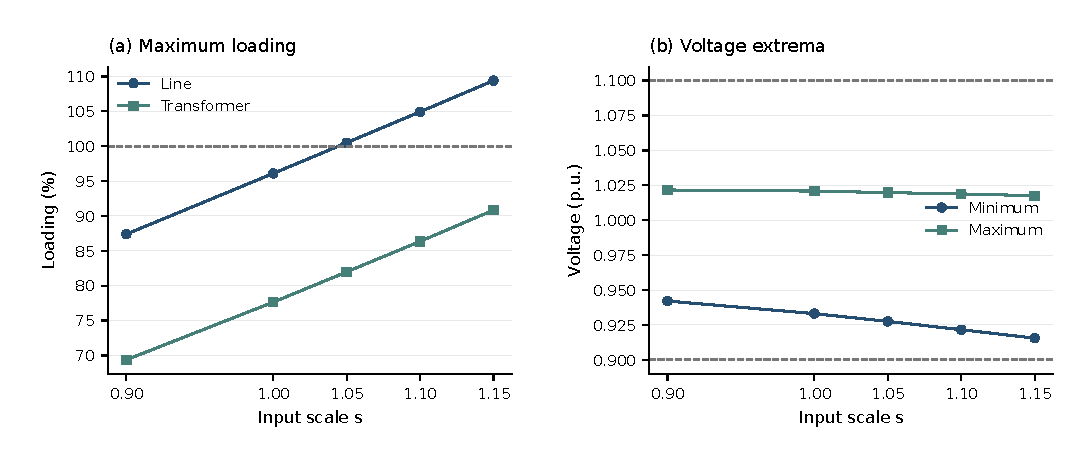
\includegraphics[keepaspectratio]{figures_final/fig11_grid_stress.pdf}}

\textbf{Figure S3 \textbar{} Deterministic grid-stress response.}
Maximum line and transformer loading and minimum and maximum bus
voltage. Dashed lines mark 100\% line loading and the 0.90--1.10 p.u.
screening band.

Six times are selected in advance: maximum and minimum load, maximum
wind, maximum photovoltaic generation, maximum net import, and maximum
net export. The same 1,649 contingencies are applied at every time in
N1-3787. The panel contains 9,894 cases, of which 9,888 converge under
the principal solution. Absolute screening passes 6,048 cases; 9,064
cases have neither a new violation relative to N−0 nor a material
island. The latter metric does not detect every worsening of a
pre-existing violation and does not replace absolute criteria.

\pandocbounded{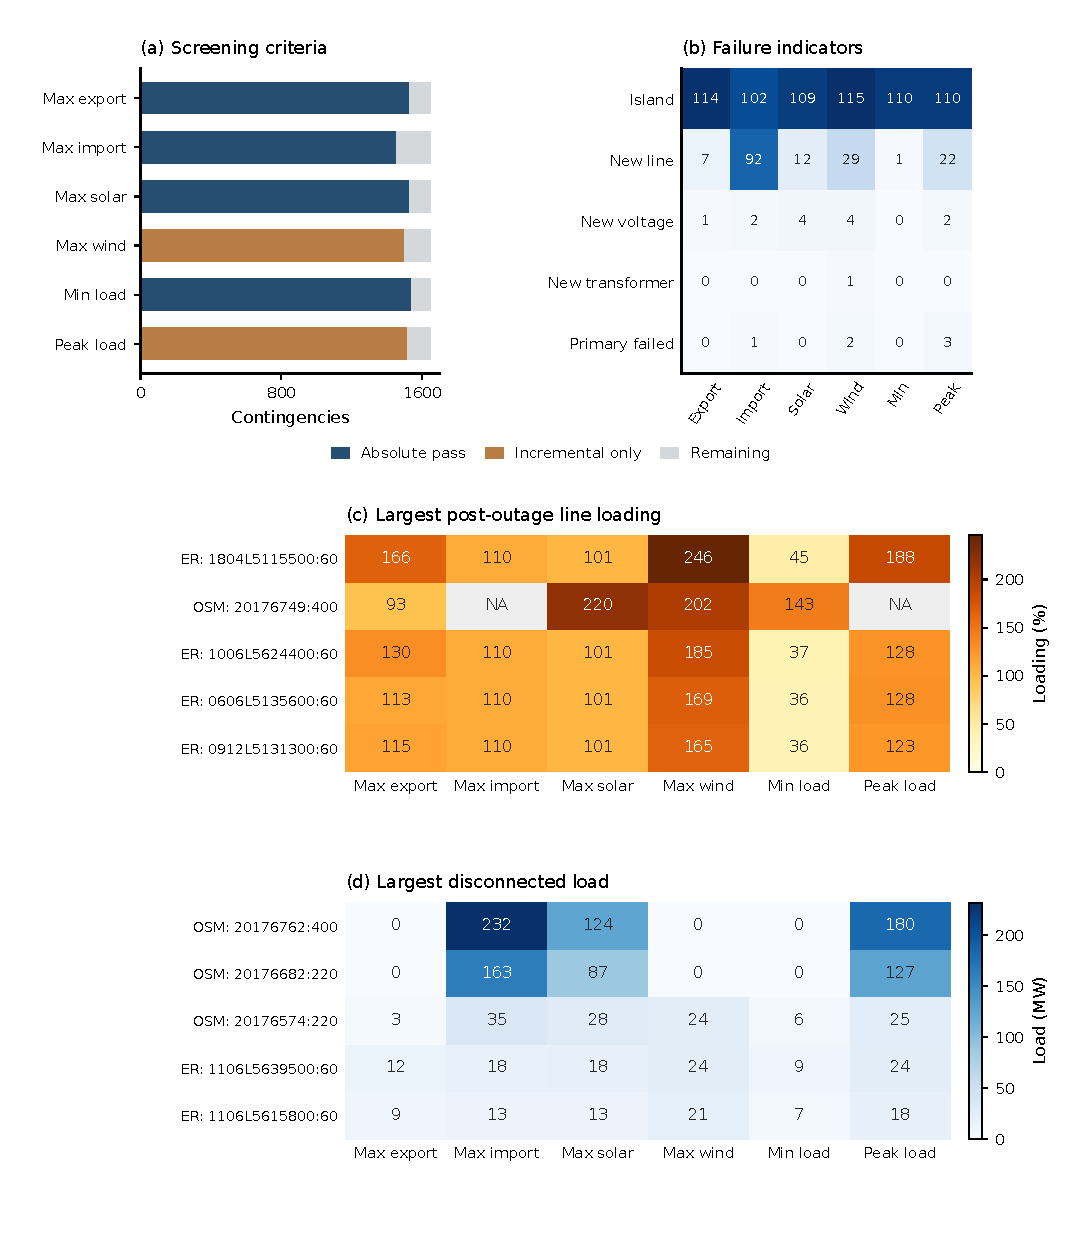
\includegraphics[keepaspectratio]{figures_final/fig12_annual_nminus1.pdf}}

\textbf{Figure S4 \textbar{} Full-element N−1 screening at
representative times.} Absolute and incremental diagnostics, material
islands, new violations, principal-solution failures, and the elements
associated with the largest loading and disconnected load.

\textbf{Table S10 \textbar{} Full-element N−1 results at six
representative times.}

\begin{longtable}[]{@{}
  >{\raggedright\arraybackslash}p{(\linewidth - 10\tabcolsep) * \real{0.1304}}
  >{\raggedleft\arraybackslash}p{(\linewidth - 10\tabcolsep) * \real{0.1739}}
  >{\raggedleft\arraybackslash}p{(\linewidth - 10\tabcolsep) * \real{0.1739}}
  >{\raggedleft\arraybackslash}p{(\linewidth - 10\tabcolsep) * \real{0.1739}}
  >{\raggedleft\arraybackslash}p{(\linewidth - 10\tabcolsep) * \real{0.1739}}
  >{\raggedleft\arraybackslash}p{(\linewidth - 10\tabcolsep) * \real{0.1739}}@{}}
\toprule\noalign{}
\begin{minipage}[b]{\linewidth}\raggedright
Snapshot
\end{minipage} & \begin{minipage}[b]{\linewidth}\raggedleft
Cases
\end{minipage} & \begin{minipage}[b]{\linewidth}\raggedleft
Principal solution converged
\end{minipage} & \begin{minipage}[b]{\linewidth}\raggedleft
Absolute screen passed
\end{minipage} & \begin{minipage}[b]{\linewidth}\raggedleft
No new violation and no material island
\end{minipage} & \begin{minipage}[b]{\linewidth}\raggedleft
Material island
\end{minipage} \\
\midrule\noalign{}
\endhead
\bottomrule\noalign{}
\endlastfoot
Maximum net export & 1,649 & 1,649 & 1,527 & 1,527 & 114 \\
Maximum net import & 1,649 & 1,648 & 1,455 & 1,455 & 102 \\
Maximum photovoltaic & 1,649 & 1,649 & 1,526 & 1,526 & 109 \\
Maximum wind & 1,649 & 1,647 & 0 & 1,502 & 115 \\
Minimum load & 1,649 & 1,649 & 1,538 & 1,538 & 110 \\
Maximum load & 1,649 & 1,646 & 2 & 1,516 & 110 \\
Total & 9,894 & 9,888 & 6,048 & 9,064 & 660 \\
\end{longtable}

The last three diagnostic columns are computed separately and are not
mutually exclusive exhaustive classes. At maximum net export, eight
additional non-islanding cases have new violations: seven line-thermal
and one voltage violation. Together with 1,527 no-new-violation cases
and 114 material islands, they account for all 1,649 cases.

\end{document}
